% ---------------------------------------------------------------- Figure ----
% Annotated capture of the running product: the rubric evidence review.
% This is a screenshot of working software, not a mockup.
\begin{figure}[htbp]
\centering

\begin{tikzpicture}[
  font=\fontsize{8}{9.5}\selectfont,
  pin/.style={
    circle, draw=white, fill=uired, text=white, line width=0.9pt,
    minimum size=0.38cm, inner sep=0pt,
    font=\fontsize{7}{7}\selectfont\bfseries
  }
]

\node[inner sep=0pt, outer sep=0pt] (shot)
  {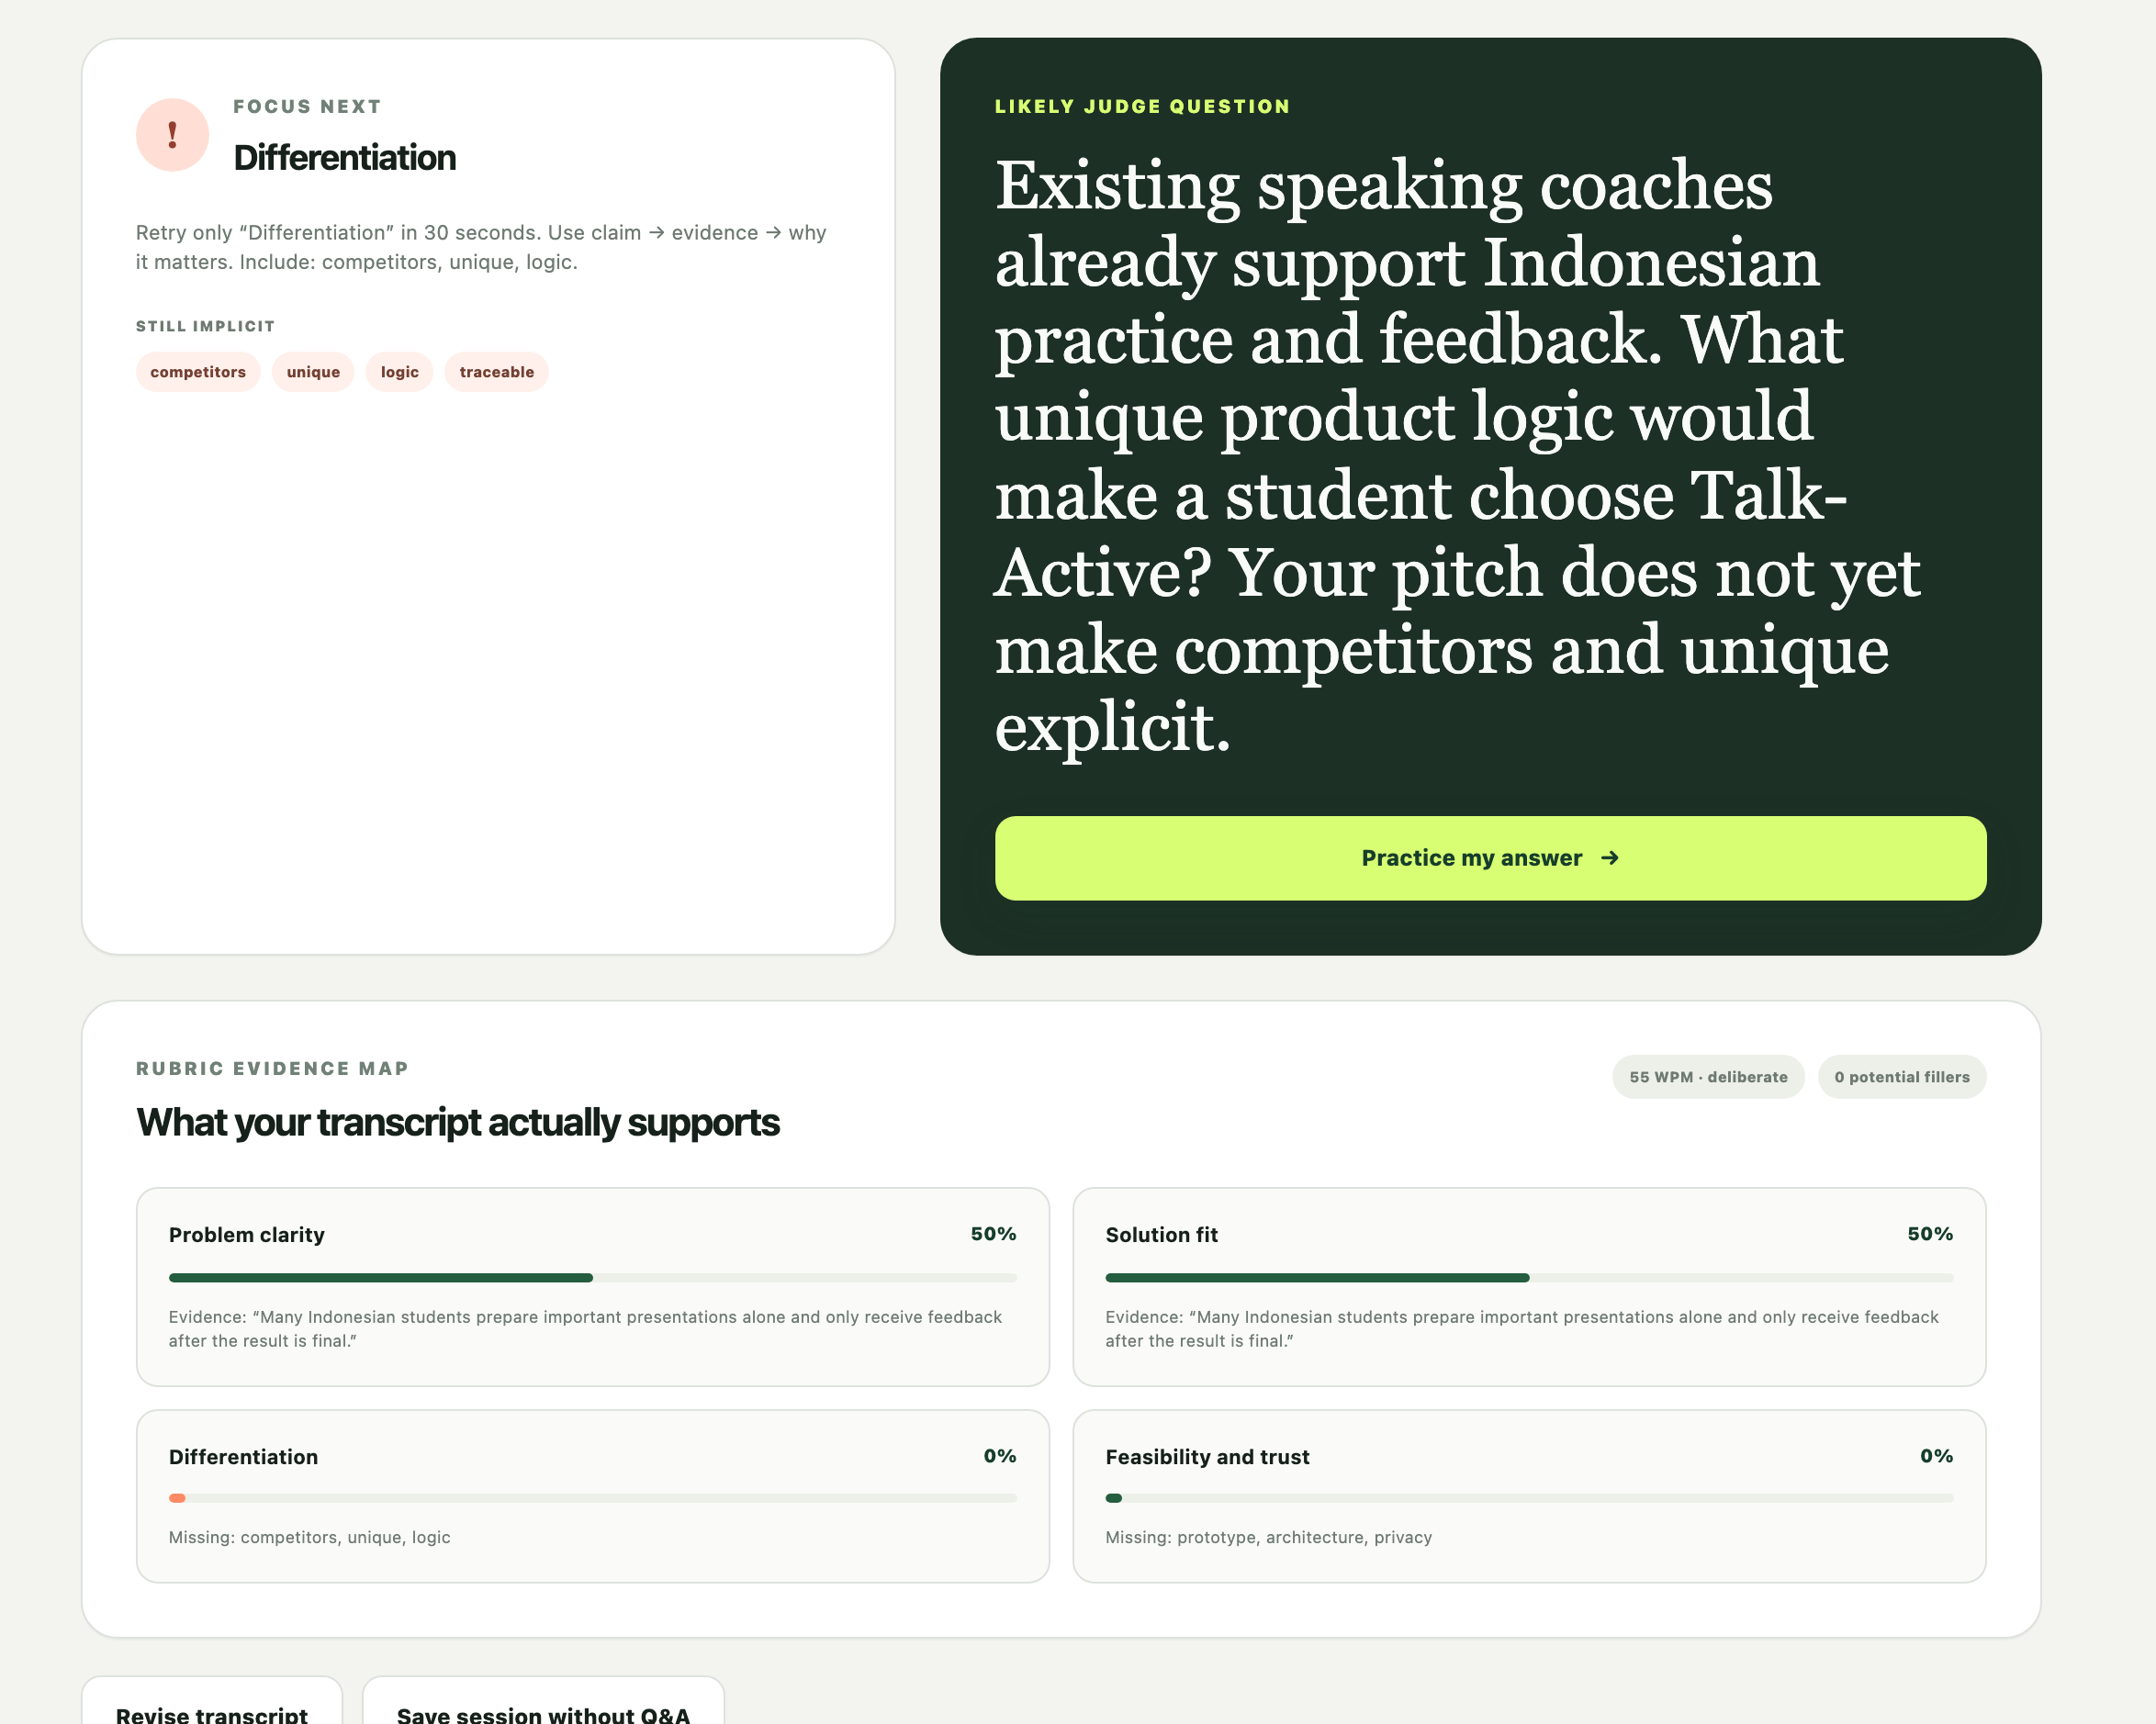
\includegraphics[width=0.66\textwidth]{assets/screens/crop-evidence.png}};

% normalised overlay coordinate system across the image node
\begin{scope}[
  x={($(shot.south east)-(shot.south west)$)},
  y={($(shot.north west)-(shot.south west)$)},
  shift={(shot.south west)}
]
  \node[pin] at (0.048,0.905) {1};
  \node[pin] at (0.048,0.775) {2};
  \node[pin] at (0.505,0.905) {3};
  \node[pin] at (0.048,0.395) {4};
  \node[pin] at (0.048,0.118) {5};
\end{scope}

\draw[rulegrey, line width=0.5pt] (shot.south west) rectangle (shot.north east);

\end{tikzpicture}

\caption{The rubric evidence review, captured from the running prototype.
\textbf{(1)}~the weakest criterion is named, not a vague weakness;
\textbf{(2)}~the evidence still missing is listed as cues to make explicit;
\textbf{(3)}~the judge question is generated from that criterion;
\textbf{(4)}~every criterion cites the exact transcript sentence behind its
verdict; \textbf{(5)}~unsupported criteria name precisely what was absent. This
screen is why \ProductName{} is not a speaking coach: every statement it makes
is anchored to a criterion the evaluator wrote and a sentence the student said.}
\label{fig:mockup}
\end{figure}
